%%%%%%%%%%%%%%%%%%%%%%%%%%%%%%%%%%%%%%%%%%%%%%%%%%%%%%%%%%%%%%%%%%%%%%%
% Vorlage für Bachelor- und Masterarbeiten mit pdflatex nach dem Layout des ITS
% Fabian Bleier (fabian.bleier@kit.edu), September 2016
%%%%%%%%%%%%%%%%%%%%%%%%%%%%%%%%%%%%%%%%%%%%%%%%%%%%%%%%%%%%%%%%%%%%%%%
% Kurzbeschreibung
% Der Hauptordner enthält in erster Linie das Dokument "gesamt.tex". Dieses enthält wiederum alle notwendigen Nutzereingaben (Autor, Titel etc.). 
% Die einzelnen Kapitel werden in das Gesamtdokument eingeladen und liegen im Ordner "kapitel". 
% Der Ordner "sonstiges" enthält alle Seiten außerhalb des eigentlichen Textkörpers (Formatierung der Kopfzeilen, Deckblätter, die einzubindenden Pakete, Institutslogos, Macros, Verzeichnisse usw.)
% Der Ordner "literatur" enthält alle Dateien, welche zur Gestaltung eines Literaturverzeichnisses notwendig sind (Die bibtex-Datei, die bst-Datei, und das eigentliche Verzeichnis).
% Im Ordner "bilder" können alle Abbildungen abgelegt werden.
% Der Ordner "dokumentation" enthält verschiedene Dokumentationen zu den verwendeten Paketen, ferner eine ausbaufähige Dokumentation des LaTeX-Dokuments

%%%%%%%%%%%%%%%%%%%%%%%%%%%%%%%%%%%%%%%%%%%%%%%%%%%%%%%%%%%%%%%%%%%%%%%
% Dokumenterstellung
%%%%%%%%%%%%%%%%%%%%%%%%%%%%%%%%%%%%%%%%%%%%%%%%%%%%%%%%%%%%%%%%%%%%%%%
\documentclass[
paper=a4,										% Seitenformat
12pt,											% Schriftgröße
twoside=false,									% zweiseitig true/false
headings=small,									% Formatierung der Überschriften
draft=false,									% Entwurfsmodus true/false
]{scrreprt}										% KOMA-Klasse Report
%\usepackage{showframe}							% Schriftfeld in Dokument anzeigen

%%%%%%%%%%%%%%%%%%%%%%%%%%%%%%%%%%%%%%%%%%%%%%%%%%%%%%%%%%%%%%%%%%%%%%%
% Metadaten und Variablen zur Verwendung im Dokument und zur Erstellung der PDF-Datei
%%%%%%%%%%%%%%%%%%%%%%%%%%%%%%%%%%%%%%%%%%%%%%%%%%%%%%%%%%%%%%%%%%%%%%%
\newcommand{\doctitle}{Numerische Untersuchung der Str\"omung durch rotierende Bohrungen} 				% Titel der Arbeit
\newcommand{\doctype}{Bachelorarbeit}			% Dokumenttyp
\newcommand{\docauthor}{Egon Eiermann, B.Sc.}	% Autor
\newcommand{\doclocation}{Karlsruhe}			% Erstellungsort
\newcommand{\betreuerI}{Max Mustermann, M.Sc.}	% Betreuer1
\newcommand{\betreuerII}{}						% Betreuer2 (optional, kann leer gelassen werden)
\newcommand{\docsubject}{Kurzbeschreibung}		% Kurzbeschreibung
\newcommand{\dockeywords}{%
Flugzeugtriebwerke,
	Gasturbinen, 
	W\"arme\"ubergang
}												% Stichworte
\newcommand{\doccreator}{pdflatex}				% Erstellt mit
\newcommand{\docproducer}{LaTeX}				% Software
\newcommand{\docdate}{\today}					% Erstellungsdatum

%%%%%%%%%%%%%%%%%%%%%%%%%%%%%%%%%%%%%%%%%%%%%%%%%%%%%%%%%%%%%%%%%%%%%%%
% Formatierung, Pakete, Makros einbinden
%%%%%%%%%%%%%%%%%%%%%%%%%%%%%%%%%%%%%%%%%%%%%%%%%%%%%%%%%%%%%%%%%%%%%%%
%%%%%%%%%%%%%%%%%%%%%%%%%%%%%%%%%%%%%%%%%%%%%%%%%%%%%%%%%%%%%%%%%%%%%%%%%%%%%%%%%%%%%%%%
% Standardpakete
% Hilfe zu Paketen bieten die Kommandozeilentools texdoc (TeXLive) bzw. mthelp (Miktex)
%%%%%%%%%%%%%%%%%%%%%%%%%%%%%%%%%%%%%%%%%%%%%%%%%%%%%%%%%%%%%%%%%%%%%%%%%%%%%%%%%%%%%%%%
\usepackage[comma,
	sort,
% square,
%	numbers
	]{natbib}									% Formatierung des Literaturverzeichnisses 
\usepackage[ngerman,english]{babel} 			% Sprachpaket: neudeutsch, englisch, französisch
\usepackage[utf8]{inputenc}        				% Standardpackage: unterstützt Zeichentabellen
\usepackage[T1]{fontenc}              			% Standardpackage: unterstützt Schriftauswahl
\usepackage{lmodern}							% Schrift latin modern
\usepackage{amsmath}                  			% Standardpackage: Formelformatierung
\usepackage{amsfonts}                 			% Standardpackage: Formelformatierung
\usepackage{amssymb}                  			% Standardpackage: Formelformatierung
\usepackage{mathptmx}   						% Formeln und Text mit Adobe Times Roman Postscript-Schriften
\usepackage[scaled=.92]{helvet}					% Helvetica ist serifenlose Standardschriftart
\usepackage{courier}							% Courier ist typeset Standardschriftart
\usepackage{fixmath}   							% ISO-Formatierung griechischer Buchstaben
\usepackage[headsepline
	]{scrlayer-scrpage}							% Header-Formatierung
\usepackage{siunitx}                  			% Formatierung der Einheiten
\sisetup{
	per-mode=symbol,							% Form des Bruchstrichs: reciprocal (Exponent), symbol (/) oder fraction
	locale = DE 								% Ländereinstellung (Dezimaltrennzeichen usw.)
}
\usepackage{graphicx}							% Zusätzliche Optionen zur Grafikeinbindung
%\graphicspath{{./bilder/}]}

%%%%%%%%%%%%%%%%%%%%%%%%%%%%%%%%%%%%%%%%%%%%%%%%%%%%%%%%%%%%%%%%%%%%%%%%%%%%%%%%%%
% Zusätzliche Pakete
%%%%%%%%%%%%%%%%%%%%%%%%%%%%%%%%%%%%%%%%%%%%%%%%%%%%%%%%%%%%%%%%%%%%%%%%%%%%%%%%%%
\usepackage[
	margin=10pt,
	labelformat=simple,
	labelsep=colon,
	font=normal,
	labelfont=normal,
	skip=15pt
	]{caption}[2008/08/24]  					% Erlaubt die Formatierung der Bildunter- und Tabellenüberschriften
\usepackage{ifthen}								% Paket für Abfragen
\usepackage{color}								% Farbige Texte
\usepackage{transparent}						% Transparenz
\usepackage{booktabs}							% Nützliche Tabellentools (\topline, \midline, \bottomline, ...)
\usepackage{longtable}							% Tabellen über mehrere Seiten

%%%%%%%%%%%%%%%%%%%%%%%%%%%%%%%%%%%%%%%%%%%%%%%%%%%%%%%%%%%%%%%%%%%%%%%%%%%%%%%%%%
% Optionale (aber evtl. nützliche) Pakete
%%%%%%%%%%%%%%%%%%%%%%%%%%%%%%%%%%%%%%%%%%%%%%%%%%%%%%%%%%%%%%%%%%%%%%%%%%%%%%%%%%
\usepackage{lipsum}								% Einbindung von Lorem Ipsum als Platzhalter
\usepackage{multirow}                 			% Befehle analog \multicolumn in vertikaler Richtung
\usepackage{subcaption}							% Ermöglicht die Verwendung von subfigure
\PreventPackageFromLoading{subfig} 				% Verhindert das Laden des veralteten Packages subfig
\usepackage[svgpath=bilder/]{svg}	  			% Automatisches Einbinden von svg-Dateien
\usepackage{textcomp}							% Ermöglicht die Einbindung von Symbolen
\usepackage[
	colorlinks=true, 
	linkcolor=black, 
	citecolor=black, 
	urlcolor=black
	]{hyperref}									% Verlinkte Referenzen
\hypersetup{
	pdftitle={\doctitle},
	pdfsubject={\docsubject},
	pdfauthor={\docauthor},
	pdfkeywords={\dockeywords},
  pdfcreator={\doccreator},
  pdfproducer={\docproducer}
}
\usepackage{nameref}							% Definition der Metadaten, die dem PDF-Dokument hinterlegt werden
\usepackage[nonumberlist,
	nomain=true,
	acronym,
	toc,
	numberedsection=false,
	]{glossaries}								% Glossaries-Paket zur Erstellung eines Glossars
\newcounter{dummy} 								% korrekte Verlinkung der Literatur und anderer Verzeichnisse					% Pakete
%%%%%%%%%%%%%%%%%%%%%%%%%%%%%%%%%%%%%%%%%%%%%%%%%%%%%%%%%%%%%%%%%%%%%%%
% Zuweisen von Zahlenwerten zu Monatsnamen 
%%%%%%%%%%%%%%%%%%%%%%%%%%%%%%%%%%%%%%%%%%%%%%%%%%%%%%%%%%%%%%%%%%%%%%%
\newcommand{\monthword}[1]{\ifcase#1\or Januar\or Februar\or M\"arz\or April\or
                                        Mai\or Juni\or Juli\or August\or
                                        September\or Oktober\or November\or Dezember\fi}
																				
%%%%%%%%%%%%%%%%%%%%%%%%%%%%%%%%%%%%%%%%%%%%%%%%%%%%%%%%%%%%%%%%%%%%%%%%%%%%%%%%%%%%%%%%%
% Benutzerdefinierte Übersetzungen (Fixed names und Variablen)
%%%%%%%%%%%%%%%%%%%%%%%%%%%%%%%%%%%%%%%%%%%%%%%%%%%%%%%%%%%%%%%%%%%%%%%%%%%%%%%%%%%%%%%%%
% Definieren von neuen Namen für die einzelnen Tabellen
\newcommand{\latinsymbolsname}{}
\newcommand{\greeksymbolsname}{}
\newcommand{\indicesname}{}
\newcommand{\simparsname}{}
\newcommand{\abbrevsname}{}
\newcommand{\unitname}{}
\newcommand{\descname}{}
% ngerman
\addto\captionsngerman{
  \renewcommand{\indexname}{Symbolverzeichnis}
  \renewcommand{\refname}{Literaturverzeichnis}
	\renewcommand{\latinsymbolsname}{Lateinische~Symbole}
	\renewcommand{\greeksymbolsname}{Griechische~Symbole}
	\renewcommand{\indicesname}{Indizes}
	\renewcommand{\simparsname}{Ähnlichkeitskennzahlen}
	\renewcommand{\abbrevsname}{Abkürzungen}
	\renewcommand{\symbolname}{Formelzeichen}
	\renewcommand{\unitname}{Einheit}
	\renewcommand{\descname}{Beschreibung}
}
% german (Verwendung wird nicht empfohlen)
\addto\captionsgerman{
  \renewcommand{\indexname}{Symbolverzeichnis}
  \renewcommand{\refname}{Literaturverzeichnis}
	\renewcommand{\latinsymbolsname}{Lateinische~Symbole}
	\renewcommand{\greeksymbolsname}{Griechische~Symbole}
	\renewcommand{\indicesname}{Indizes}
	\renewcommand{\simparsname}{Ähnlichkeitskennzahlen}
	\renewcommand{\abbrevsname}{Abkürzungen}
	\renewcommand{\symbolname}{Formelzeichen}
	\renewcommand{\unitname}{Einheit}
	\renewcommand{\descname}{Beschreibung}
}
% english (Verwendung wird nicht empfohlen)
\addto\captionsenglish{
  \renewcommand{\indexname}{List of Symbols}
  \renewcommand{\latinsymbolsname}{Latin~symbols}
	\renewcommand{\greeksymbolsname}{Greek~symbols}
	\renewcommand{\indicesname}{Indices}
	\renewcommand{\simparsname}{Similarity parameters}
	\renewcommand{\abbrevsname}{Abbreviations}
	\renewcommand{\symbolname}{Symbol}
	\renewcommand{\unitname}{Unit}
	\renewcommand{\descname}{Description}
}
% french (Verwendung wird nicht empfohlen)
\addto\captionsfrench{
  \renewcommand{\indexname}{Table de Symboles}
  \renewcommand{\latinsymbolsname}{Lettres~latines}
	\renewcommand{\greeksymbolsname}{Lettres~grecques}
	\renewcommand{\indicesname}{Indices}
	\renewcommand{\simparsname}{Nombres sans dimension}
	\renewcommand{\abbrevsname}{Abréviations}
	\renewcommand{\symbolname}{Symbol}
	\renewcommand{\unitname}{Unité}
	\renewcommand{\descname}{Description}
}

%%%%%%%%%%%%%%%%%%%%%%%%%%%%%%%%%%%%%%%%%%%%%%%%%%%%%%%%%%%%%%%%%%%%%%%%%%%%%%%%%%%%%%%%%%
%% Glossardateien erstellen
%%%%%%%%%%%%%%%%%%%%%%%%%%%%%%%%%%%%%%%%%%%%%%%%%%%%%%%%%%%%%%%%%%%%%%%%%%%%%%%%%%%%%%%%%%
%% Indexdateien für Symbolverzeichnis erstellen
%% \newglossary[Dateiendung Protokolldatei]{Typ des Glossars}{Dateiendung für Eingabedatei VOR Verarbeitung}{Dateiendung für Eingabedatei NACH Verarbeitung}{Titel}
%\newglossary[slg1]{latinSymb}{syi1_temp}{syg1}{\latinsymbolsname}
%\newglossary[slg2]{greekSymb}{syi2_temp}{syg2}{\greeksymbolsname}
%\newglossary[slg3]{simPar}{syi3_temp}{syg3}{\simparsname}
%\newglossary[slg4]{indices}{syi4_temp}{syg4}{\indicesname}
%\newglossary[slg5]{abbrevs}{syi5_temp}{syg5}{\abbrevsname}
%% Hinzufügen des Eintrags unit{}, damit eine Einheit angegeben werden kann.
%\glsaddkey{unit}{\glsentrytext{\glslabel}}{\glsentryunit}{\GLsentryunit}{\glsunit}{\Glsunit}{\GLSunit}
%\makeglossaries					% Selbstgeschriebene Macros
%%%%%%%%%%%%%%%%%%%%%%%%%%%%%%%%%%%%%%%%%%%%%%%%%%%%%%%%%%%%%%%%%%%%%%%%%%%%%%%%%%%%%%%%%
% Allgemein
%%%%%%%%%%%%%%%%%%%%%%%%%%%%%%%%%%%%%%%%%%%%%%%%%%%%%%%%%%%%%%%%%%%%%%%%%%%%%%%%%%%%%%%%%
\setlength{\unitlength}{1truecm}					% Maßeinheit fuer Bildgroessen etc. 1cm
\hyphenation{Sys-tem Sys-tems Ver-läss-lich-keit} 	% Trennhilfen einfügen

%%%%%%%%%%%%%%%%%%%%%%%%%%%%%%%%%%%%%%%%%%%%%%%%%%%%%%%%%%%%%%%%%%%%%%%%%%%%%%%%%%%%%%%%%
% Unterdrückung von Warnmeldungen (insbesondere 'overfull boxes')
%%%%%%%%%%%%%%%%%%%%%%%%%%%%%%%%%%%%%%%%%%%%%%%%%%%%%%%%%%%%%%%%%%%%%%%%%%%%%%%%%%%%%%%%%
\hfuzz2pt
\vfuzz6pt
\hbadness=10000
\vbadness=10000
%\pdfsuppresswarningpagegroup=1

%%%%%%%%%%%%%%%%%%%%%%%%%%%%%%%%%%%%%%%%%%%%%%%%%%%%%%%%%%%%%%%%%%%%%%%%%%%%%%%%%%%%%%%%%
% Textspiegel
%%%%%%%%%%%%%%%%%%%%%%%%%%%%%%%%%%%%%%%%%%%%%%%%%%%%%%%%%%%%%%%%%%%%%%%%%%%%%%%%%%%%%%%%%
\setlength{\headheight}{18pt}     					% Höhe der Kopfzeile
\setlength{\textheight}{24.0cm}              		% Texthöhe
\setlength{\textwidth}{16.0cm}               		% Textbreite
\setlength{\topmargin}{-1.0cm}               		% oberen Seitenrand festlegen, bzw. verschieben
\setlength{\oddsidemargin}{0.2cm}            		% Seitenrand anpassen -> ungerade Seiten !
\setlength{\evensidemargin}{-0.2cm}          		% Seitenrand anpassen -> gerade Seiten !
\setlength{\parindent}{0pt}                  		% Einzug bei neuen Absätzen
\setlength{\parskip}{5pt plus 2pt minus 1pt} 		% Abstand zwischen zwei Absätzen
\renewcommand{\baselinestretch}{1.1}         		% Veränderung des Zeilenabstandes {Faktor}
\setlength\itemsep{0.25\parsep}						% In Listen zwischen den Elementen 25% des Platzes zwischen zwei Absaetzen lassen.
\addtolength\footskip{0.5truecm}					% Zwischen Text und Fussnoten 5 mm mehr Abstand

%%%%%%%%%%%%%%%%%%%%%%%%%%%%%%%%%%%%%%%%%%%%%%%%%%%%%%%%%%%%%%%%%%%%%%%%%%%%%%%%%%%%%%%%%
% Einbettung von Gleitobjekten (Bilder, Tabellen etc.)
%%%%%%%%%%%%%%%%%%%%%%%%%%%%%%%%%%%%%%%%%%%%%%%%%%%%%%%%%%%%%%%%%%%%%%%%%%%%%%%%%%%%%%%%%
\setcounter{topnumber}{2} 							% ueber dem Text duerfen max. 2 Bilder stehen
\setcounter{dbltopnumber}{2}    					% für zweispaltige Seiten
\setcounter{bottomnumber}{2}						% unter dem Text duerfen max. 2 Bilder stehen
\setcounter{totalnumber}{4}							% auf jeder Seite duerfen max. 4 Bilder stehen
\renewcommand{\topfraction}{0.99}					% ueber dem Text darf max. 99% der Seite fuer Bilder verbraucht werden
\renewcommand{\dbltopfraction}{0.99} 				% zweispaltig
\renewcommand{\bottomfraction}{0.99}				% unter dem Text darf max. 99% der Seite fuer Bilder verbraucht werden
\renewcommand{\textfraction}{0.01}					% insgesamt sollte auf jeder Seite 1% Text stehen
\renewcommand{\floatpagefraction}{0.99}				% Mindestfuellgrad der Seite, wenn die Bilder auf einer separaten Bild-Seite stehen sollen
\renewcommand{\dblfloatpagefraction}{0.99}			% zweispaltig

%%%%%%%%%%%%%%%%%%%%%%%%%%%%%%%%%%%%%%%%%%%%%%%%%%%%%%%%%%%%%%%%%%%%%%%%%%%%%%%%%%%%%%%%%
% Inhaltsverzeichnis
%%%%%%%%%%%%%%%%%%%%%%%%%%%%%%%%%%%%%%%%%%%%%%%%%%%%%%%%%%%%%%%%%%%%%%%%%%%%%%%%%%%%%%%%%
\setcounter{secnumdepth}{2}                  		% Schachtelungstiefe Ueberschriften
\setcounter{tocdepth}{2}                     		% Schachtelungstiefe Eintraege im Inhaltsverzeichnis
\setkomafont{chapterentry}{\bfseries}				% Schriftart der Kapiteleinträge

%%%%%%%%%%%%%%%%%%%%%%%%%%%%%%%%%%%%%%%%%%%%%%%%%%%%%%%%%%%%%%%%%%%%%%%%%%%%%%%%%%%%%%%%%
% Überschriften formatieren
% KOMA-Font-Einstellungen
%%%%%%%%%%%%%%%%%%%%%%%%%%%%%%%%%%%%%%%%%%%%%%%%%%%%%%%%%%%%%%%%%%%%%%%%%%%%%%%%%%%%%%%%%
\makeatletter
	\renewcommand\section{\@startsection
		{section}{1}{0pt}% 								% Name, Ebene, Einzug
	  {-3.5ex \@plus -1ex \@minus -.2ex}%				% Abstand vor
 	  {2.3ex \@plus.2ex}%								% Abstand nach
		{\large \bfseries \rmfamily}}					% Layout
\makeatother
\setkomafont{chapter}{\Large \bfseries}							% Chapter layout
\setkomafont{subsection}{\large \bfseries \rmfamily}			% Subsection layout
\setkomafont{subsubsection}{\normalsize \bfseries \rmfamily}	% Subsubsection layout
\setkomafont{minisec}{\normalsize \bfseries \rmfamily}			% Minisection layout
\setkomafont{paragraph}{\normalsize \bfseries \rmfamily}		% paragraph layout
\setkomafont{subparagraph}{\normalsize \bfseries \rmfamily}		% subparagraph layout
\renewcommand*{\chapterheadstartvskip}{\vspace*{-20pt}} 		% Abstand vor Kapitelüberschriften: 1/3 der Satzspiegelhöhe
\renewcommand*{\chapterheadendvskip}{\vspace{15pt}} 			% Abstand nach Kapitelüberschriften: 3 Zeilen					% Dokumentformatierung
%%%%%%%%%%%%%%%%%%%%%%%%%%%%%%%%%%%%%%%%%%%%%%%%%%%%%%%%%%%%%%%%%%%%%%%%%%%%%%%%%%%%%%%%
% Header formatieren
%%%%%%%%%%%%%%%%%%%%%%%%%%%%%%%%%%%%%%%%%%%%%%%%%%%%%%%%%%%%%%%%%%%%%%%%%%%%%%%%%%%%%%%%
% Festlegen des Stils
\pagestyle{scrheadings}
% Formatieren der angezeigten Kapitelüberschrift (Weglassen der Kapitelnummer)
\renewcommand*{\chaptermarkformat}{}
% Festlegen des Inhalts für Abschnittskopfzeile
\automark[section]{chapter}
\clearpairofpagestyles

% Formatierung der Kopfzeilen (o = outer, i = inner), optionales Argument wird für \pagestyle{plain} gesetzt
\ohead{\pagemark}
\ihead{\headmark}
\chead{}

% Formatierung der Fußzeilen (s.o.)
\ifoot{}
\ofoot{}
\cfoot{}

% Schriftgröße/-art
\setkomafont{pageheadfoot}{\normalsize}
				% Kopf- und Fußzeilenformatierung

%%%%%%%%%%%%%%%%%%%%%%%%%%%%%%%%%%%%%%%%%%%%%%%%%%%%%%%%%%%%%%%%%%%%%%%
%	Textkörper 
%%%%%%%%%%%%%%%%%%%%%%%%%%%%%%%%%%%%%%%%%%%%%%%%%%%%%%%%%%%%%%%%%%%%%%%
\begin{document}

%%%%%%%%%%%%%%%%%%%%%%%%%%%%%%%%%%%%%%%%%%%%%%%%%%%%%%%%%%%%%%%%%%%%%%%
% Sprachauswahl
%%%%%%%%%%%%%%%%%%%%%%%%%%%%%%%%%%%%%%%%%%%%%%%%%%%%%%%%%%%%%%%%%%%%%%%
% neudeutsch = {ngerman}, englisch = {english}, französisch = {french}
\selectlanguage{ngerman}

%%%%%%%%%%%%%%%%%%%%%%%%%%%%%%%%%%%%%%%%%%%%%%%%%%%%%%%%%%%%%%%%%%%%%%%
% Titelseiten, Inhaltsverzeichnis, Tabellenverzeichnis
%%%%%%%%%%%%%%%%%%%%%%%%%%%%%%%%%%%%%%%%%%%%%%%%%%%%%%%%%%%%%%%%%%%%%%%
%%%%%%%%%%%%%%%%%%%%%%%%%%%%%%%%%%%%%%%%%%%%%%%%%%%%%%%%%%%%%%%%%%%%%%%%%%%%%%%%%%%%%%%%
% Titelseiten (Deckblatt und eidesstattliche Versicherung)
%%%%%%%%%%%%%%%%%%%%%%%%%%%%%%%%%%%%%%%%%%%%%%%%%%%%%%%%%%%%%%%%%%%%%%%%%%%%%%%%%%%%%%%%
\pagenumbering{alph}							% Seitennummerierung mittels Buchstaben
%%%%%%%%%%%%%%%%%%%%%%%%%%%%%%%%%%%%%%%%%%%%%%%%%%%%%%%%%%%%%%%%
% Titelseite basierend auf dem Entwurf von Pascal Schuler vom 01.12.2009
%%%%%%%%%%%%%%%%%%%%%%%%%%%%%%%%%%%%%%%%%%%%%%%%%%%%%%%%%%%%%%%%
\begin{titlepage}
\pagestyle{empty}												
%%%%%%%%%%%%%%%%%%%%%%%%%%%%%%%%%%%%%%%%%%%%%%%%%%%%%%%%%%%%%%%%
% Instituts-/KIT-Logo
%%%%%%%%%%%%%%%%%%%%%%%%%%%%%%%%%%%%%%%%%%%%%%%%%%%%%%%%%%%%%%%%
\hspace*{-1cm}													% gesamte Titelseite um 1cm nach rechts verschieben
\parbox[t][21cm][t]{4cm}										% zwischen den parbox'n darf keine Leerzeile existieren
	{															% sonst werden sie untereinander statt nebeneinander gestellt	
	\begin{center}
		\vspace*{-2cm}\hspace*{-2cm}
		
\includegraphics[scale=1.0]{sonstiges/its_logo.png}		% LOGO des ITS
		
		\vspace*{21cm}\hspace*{0cm}
		
\includegraphics[scale=0.6]{sonstiges/kit_logo.pdf}		% KIT-Logo
	\end{center}
	}
%%%%%%%%%%%%%%%%%%%%%%%%%%%%%%%%%%%%%%%%%%%%%%%%%%%%%%%%%%%%%%%%
% Institutssymbol
%%%%%%%%%%%%%%%%%%%%%%%%%%%%%%%%%%%%%%%%%%%%%%%%%%%%%%%%%%%%%%%%
\parbox[t][22cm][t]{12cm}								% parbox = 2.Spalte mit Text
{																			% [Ausrichtung] [Höhe] [AusrichtenInnen] {Breite}
\begin{flushleft}
	\vspace*{-1.6cm}\hspace*{-1.7cm}			% (2-x)cm = Abstand zwischen ITS-Logo und -Name
	\Large\sffamily
	\parbox[t][3.0cm][t]{13.5cm}
		{
			Institut~für~Thermische~Strömungsmaschinen\\
			\large Prof.~Dr.-Ing.~H.-J.~Bauer, Ord.~\\
		}
%%%%%%%%%%%%%%%%%%%%%%%%%%%%%%%%%%%%%%%%%%%%%%%%%%%%%%%%%%%%%%%%
% Titel
%%%%%%%%%%%%%%%%%%%%%%%%%%%%%%%%%%%%%%%%%%%%%%%%%%%%%%%%%%%%%%%%

	\vspace{3.5cm}\hspace*{-1.7cm}					% Leerzeile vor vertikaler Abstandsangabe notwendig
	\parbox[t][5cm][t]{13.5cm}								% [Ausrichtung] [Höhe] [AusrichtenInnen] {Breite}
		{
			\LARGE 				
			\centering\bfseries\doctitle  
		}
			
%%%%%%%%%%%%%%%%%%%%%%%%%%%%%%%%%%%%%%%%%%%%%%%%%%%%%%%%%%%%%%%%
% Autor
%%%%%%%%%%%%%%%%%%%%%%%%%%%%%%%%%%%%%%%%%%%%%%%%%%%%%%%%%%%%%%%%

	\vspace{2cm}\hspace*{-1.7cm}						% Leerzeile vor vertikaler Abstandsangabe notwendig
	\parbox[t][3cm][t]{13.5cm}
		{
			\LARGE	
			\centerline{\doctype}
			\centerline{von}
			\centerline{\bfseries\docauthor}
		} 		
\end{flushleft}
%%%%%%%%%%%%%%%%%%%%%%%%%%%%%%%%%%%%%%%%%%%%%%%%%%%%%%%%%%%%%%%%
% Betreuer
%%%%%%%%%%%%%%%%%%%%%%%%%%%%%%%%%%%%%%%%%%%%%%%%%%%%%%%%%%%%%%%%
	% Leerzeile vor vertikaler Abstandsangabe notwendig
	\ifthenelse{\equal{\betreuerII}{}}
	{
		\vspace*{2cm}\hspace*{-1.7cm}
	}
	{
		\vspace*{2cm}\vspace*{-\baselineskip}\hspace*{-1.7cm}
	}
	\parbox[t][1cm][t]{13.5cm}
	{
		\ifthenelse{\equal{\betreuerII}{}}
		{
			\leftline{\Large\sffamily Betreuer:~\bfseries\betreuerI}
		}
		{
		\begin{tabbing}
			\Large\sffamily Betreuer: \= \Large\sffamily\bfseries\betreuerI\\
			\> \Large\sffamily\bfseries\betreuerII
		\end{tabbing}
		\vspace*{-\baselineskip}
		}
		\vspace*{0.5cm}
		\hrule
		\vspace*{0.5cm}
		\leftline{\Large\sffamily \monthword{\month}~\the\year}																		
	}
}
\cleardoublepage

%%%%%%%%%%%%%%%%%%%%%%%%%%%%%%%%%%%%%%%%%%%%%%%%%%%%%%%%%%%%%%%%
%           Versicherung
%%%%%%%%%%%%%%%%%%%%%%%%%%%%%%%%%%%%%%%%%%%%%%%%%%%%%%%%%%%%%%%%
\pagestyle{empty}
\vspace*{0.1cm}
Ich versichere, die Arbeit selbständig verfasst und nur die angegebenen Quellen und Hilfsmittel verwendet zu haben. Die wörtlich oder inhaltlich übernommenen Stellen sind als solche kenntlich gemacht. Die Satzung des Karlsruher Instituts für Technologie (KIT) zur Sicherung guter wissenschaftlicher Praxis wurde von mir in der aktuellen Fassung beachtet.
\vspace*{3cm}
\begin{center}
\doclocation, \docdate
\end{center}
\cleardoublepage
\end{titlepage}

\pagenumbering{roman}							% Seitennummerierung mittels römischer Zahlen

%%%%%%%%%%%%%%%%%%%%%%%%%%%%%%%%%%%%%%%%%%%%%%%%%%%%%%%%%%%%%%%%%%%%%%%%%%%%%%%%%%%%%%%%
% Inhaltsverzeichnis
%%%%%%%%%%%%%%%%%%%%%%%%%%%%%%%%%%%%%%%%%%%%%%%%%%%%%%%%%%%%%%%%%%%%%%%%%%%%%%%%%%%%%%%%
\tableofcontents
\cleardoublepage

%%%%%%%%%%%%%%%%%%%%%%%%%%%%%%%%%%%%%%%%%%%%%%%%%%%%%%%%%%%%%%%%%%%%%%%%%%%%%%%%%%%%%%%%
% Symbolverzeichnis
%%%%%%%%%%%%%%%%%%%%%%%%%%%%%%%%%%%%%%%%%%%%%%%%%%%%%%%%%%%%%%%%%%%%%%%%%%%%%%%%%%%%%%%%
\refstepcounter{dummy}
\addcontentsline{toc}{chapter}{\indexname}		% Verzeichnisname in TOC
\chapter*{\indexname}
% Header
\begin{longtable}{@{}p{0.2\textwidth}@{}p{0.15\textwidth}@{}p{0.64\textwidth}}
\bfseries{\symbolname} & \bfseries{\unitname} & \bfseries{\descname} \\
\hline
\end{longtable}
% Einbinden des automatisch erstellten Symbolverzeichnisses (derzeit nicht möglich)
%%\deftranslation[to=ngerman]{Glossary}{Symbolverzeichnis}
%\setglossarysection{subsubsection}
\renewcommand{\glossarysection}[3][]{}
\vspace{-10pt}
%%%%%%%%%%%%%%%%%%%%%%%%%%%%%%%%%%%%%%%%%%%%%%%%%%%%%%%%%%%%%%%%%%%%%%%%%%%%%%%%%%%%%%%%%%
% Eintr�ge definieren
%%%%%%%%%%%%%%%%%%%%%%%%%%%%%%%%%%%%%%%%%%%%%%%%%%%%%%%%%%%%%%%%%%%%%%%%%%%%%%%%%%%%%%%%%%
% Lateinische Symbole
%%%%%%%%%%%%%%%%%%%%%%%%%%%%%%%%%%%%%%%%%%%%%%%%%%%%%%%%%%%%%%%%%%%%%%%%%%%%%%%%%%%%%%%%%%
\newglossaryentry{hoehe}{%
	type=latinSymb,
	name=\ensuremath{H},
	symbol = \ensuremath{H},
	description={H�he},
	unit={\si{\meter}}
}
\newglossaryentry{cp}{%
	type=latinSymb,
	name=\ensuremath{c_p},
	symbol = \ensuremath{c_p},
	description={Spezifische W�rmekapazit�t},
	unit={\si{\joule\per\kilogram\per\kelvin}}
}
\newglossaryentry{faktorxyz}{%
	type=latinSymb,
	name=\ensuremath{F_\text{xy}},
	symbol=\ensuremath{F_\text{xy}},
	description={Faktor xy},
	unit={}
}
%%%%%%%%%%%%%%%%%%%%%%%%%%%%%%%%%%%%%%%%%%%%%%%%%%%%%%%%%%%%%%%%%%%%%%%%%%%%%%%%%%%%%%%%%
% Griechische Symbole
%%%%%%%%%%%%%%%%%%%%%%%%%%%%%%%%%%%%%%%%%%%%%%%%%%%%%%%%%%%%%%%%%%%%%%%%%%%%%%%%%%%%%%%%%
\newglossaryentry{dissrate}{%
	type=greekSymb,
	name=\ensuremath{\varepsilon},
	symbol=\ensuremath{\varepsilon},
	description={Dissipationsrate},
	unit={\si{\meter^2\per\second^3}}
}
\newglossaryentry{isentropenexp}{%
	type=greekSymb,
	name=\ensuremath{\kappa},
	symbol=\ensuremath{\kappa},
	description={Isentropenexponent},
	unit={}
}
\newglossaryentry{waermeleit}{%
	type=greekSymb,
	name=\ensuremath{\lambda},
	symbol = \ensuremath{\lambda},
	description={W�rmeleitf�higkeit},
	unit={\si{\watt\per\meter\per\kelvin}}
}
%%%%%%%%%%%%%%%%%%%%%%%%%%%%%%%%%%%%%%%%%%%%%%%%%%%%%%%%%%%%%%%%%%%%%%%%%%%%%%%%%%%%%%%%%
% Indizes
%%%%%%%%%%%%%%%%%%%%%%%%%%%%%%%%%%%%%%%%%%%%%%%%%%%%%%%%%%%%%%%%%%%%%%%%%%%%%%%%%%%%%%%%%
\newglossaryentry{ind_x}{%
	type=indices,
	name=\ensuremath{\text{x}},
	symbol=\ensuremath{\text{x}},
	description={x-Koordinate},
	unit={}
}
\newglossaryentry{ind_r}{%
	type=indices,
	name=\ensuremath{\text{r}},
	symbol=\ensuremath{\text{r}},
	description={r-Koordinate},
	unit={}
}
\newglossaryentry{ind_z}{%
	type=indices,
	name=\ensuremath{\text{z}},
	symbol=\ensuremath{\text{z}},
	description={z-Koordinate},
	unit={}
}

%%%%%%%%%%%%%%%%%%%%%%%%%%%%%%%%%%%%%%%%%%%%%%%%%%%%%%%%%%%%%%%%%%%%%%%%%%%%%%%%%%%%%%%%%
% Ähnlichkeitskennzahlen
%%%%%%%%%%%%%%%%%%%%%%%%%%%%%%%%%%%%%%%%%%%%%%%%%%%%%%%%%%%%%%%%%%%%%%%%%%%%%%%%%%%%%%%%%
\newglossaryentry{sim_re}{%
	type=simPar,
	name=\ensuremath{\textit{Re}},
	symbol=\ensuremath{\textit{Re}},
	description={Reynoldszahl},
	unit={}
}
\newglossaryentry{sim_nu}{%
	type=simPar,
	name=\ensuremath{\textit{Nu}},
	symbol=\ensuremath{\textit{Nu}},
	description={Nu�eltzahl},
	unit={}
}
\newglossaryentry{sim_pr}{%
	type=simPar,
	name=\ensuremath{\textit{Pr}},
	symbol=\ensuremath{\textit{Pr}},
	description={Prandtlzahl},
	unit={}
}
\newglossaryentry{sim_bi}{%
	type=simPar,
	name=\ensuremath{\textit{Bi}},
	symbol=\ensuremath{\textit{Bi}},
	description={Biotzahl},
	unit={}
}
%%%%%%%%%%%%%%%%%%%%%%%%%%%%%%%%%%%%%%%%%%%%%%%%%%%%%%%%%%%%%%%%%%%%%%%%%%%%%%%%%%%%%%%%%
% Abk�rzungen
%%%%%%%%%%%%%%%%%%%%%%%%%%%%%%%%%%%%%%%%%%%%%%%%%%%%%%%%%%%%%%%%%%%%%%%%%%%%%%%%%%%%%%%%%
\newglossaryentry{abbr_fem}{%
	type=abbrevs,
	name=\ensuremath{\text{FEM}},
	symbol=\ensuremath{\text{FEM}},
	description={Finite-Elemente-Methode},
}
\newglossaryentry{abbr_cfd}{%
	type=abbrevs,
	name=\ensuremath{\text{CFD}},
	symbol=\ensuremath{\text{CFD}},
	description={Computational Fluid Dynamics},
}
%%%%%%%%%%%%%%%%%%%%%%%%%%%%%%%%%%%%%%%%%%%%%%%%%%%%%%%%%%%%%%%%%%%%%%%%%%%%%%%%%%%%%%%%%%
% Formatierung
%%%%%%%%%%%%%%%%%%%%%%%%%%%%%%%%%%%%%%%%%%%%%%%%%%%%%%%%%%%%%%%%%%%%%%%%%%%%%%%%%%%%%%%%%%
\newglossarystyle{symbUnit}{%
	\setglossarystyle{long3col}% base this style on the list style
	\renewenvironment{theglossary}{
		\begin{longtable}{@{}p{0.2\textwidth}@{}p{0.15\textwidth}@{}p{0.64\textwidth}}}%
		{\end{longtable}}%
	\renewcommand*{\glossaryheader}{%  Change the table header
		\multicolumn{3}{@{}l}{\itshape \glossarytitle} \\
		\endhead}
	\renewcommand*{\glossentry}[2]{%  Change the displayed items
		\glstarget{##1}{\glossentryname{##1}} %
		& \glsunit{##1}% Description
		& \glossentrydesc{##1}
		\tabularnewline}
		\vspace{-6pt}
}

%%%%%%%%%%%%%%%%%%%%%%%%%%%%%%%%%%%%%%%%%%%%%%%%%%%%%%%%%%%%%%%%%%%%%%%%%%%%%%%%%%%%%%%%%%
% Formatierung
%%%%%%%%%%%%%%%%%%%%%%%%%%%%%%%%%%%%%%%%%%%%%%%%%%%%%%%%%%%%%%%%%%%%%%%%%%%%%%%%%%%%%%%%%%
\newglossarystyle{symb}{%
	\setglossarystyle{long3col}% base this style on the list style
	\renewenvironment{theglossary}{
		\begin{longtable}{@{}p{0.2\textwidth}@{}p{0.15\textwidth}@{}p{0.64\textwidth}}}%
		{\end{longtable}}%
	\renewcommand*{\glossaryheader}{%  Change the table header
		\multicolumn{3}{@{}l}{\itshape \glossarytitle} \\
		\endhead}
	\renewcommand*{\glossentry}[2]{%  Change the displayed items
		\glstarget{##1}{\glossentryname{##1}} %
		& % Description
		& \glossentrydesc{##1}
		\tabularnewline}
		\vspace{-6pt}
}
%%%%%%%%%%%%%%%%%%%%%%%%%%%%%%%%%%%%%%%%%%%%%%%%%%%%%%%%%%%%%%%%%%%%%%%%%%%%%%%%%%%%%%%%%%
% Ausgabe
%%%%%%%%%%%%%%%%%%%%%%%%%%%%%%%%%%%%%%%%%%%%%%%%%%%%%%%%%%%%%%%%%%%%%%%%%%%%%%%%%%%%%%%%%%
\printglossary[type=latinSymb,style=symbUnit]					% Lateinische Symbole
\printglossary[type=greekSymb,style=symbUnit]					% Griechische Symbole
\printglossary[type=simPar,style=symb]								% �hnlichkeitskennzahlen
\printglossary[type=indices,style=symb]								% Indizes
\printglossary[type=abbrevs,style=symb]								% Abk�rzungen
%\printglossaries
% Einbinden des manuell erstellten Symbolverzeichnisses
\vspace{-15pt}
\begin{longtable}{@{}p{0.2\textwidth}@{}p{0.15\textwidth}@{}p{0.64\textwidth}}
%%%%%%%%%%%%%%%%%%%%%%%%%%%%%%%%%%%%%%%%%%%%%%%%%%%%%%%%%%%%%%%%%%%%%%%%%%%%%%%%%%%%%%%%%%
% Bezeichnung			&	Einheit																	& Beschreibung
%%%%%%%%%%%%%%%%%%%%%%%%%%%%%%%%%%%%%%%%%%%%%%%%%%%%%%%%%%%%%%%%%%%%%%%%%%%%%%%%%%%%%%%%%%
% Lateinische Symbole
\multicolumn{3}{@{}l}{\itshape{\latinsymbolsname}} \tabularnewline
%%%%%%%%%%%%%%%%%%%%%%%%%%%%%%%%%%%%%%%%%%%%%%%%%%%%%%%%%%%%%%%%%%%%%%%%%%%%%%%%%%%%%%%%%%
	$F_\text{xy}$	 	&   																			& Faktor xy \tabularnewline
	$H$ 						& \si{\meter}  														& Höhe \tabularnewline
	$c_p$ 					& \si{\joule\per\kilogram\per\kelvin}			& Spezifische Wärmekapazität \tabularnewline
%%%%%%%%%%%%%%%%%%%%%%%%%%%%%%%%%%%%%%%%%%%%%%%%%%%%%%%%%%%%%%%%%%%%%%%%%%%%%%%%%%%%%%%%%
% Griechische Symbole
\tabularnewline\multicolumn{3}{@{}l}{\itshape{\greeksymbolsname}} \tabularnewline
%%%%%%%%%%%%%%%%%%%%%%%%%%%%%%%%%%%%%%%%%%%%%%%%%%%%%%%%%%%%%%%%%%%%%%%%%%%%%%%%%%%%%%%%%
	$\kappa$	 			&   																			& Isentropenexponent \tabularnewline
	$\lambda$ 			& \si{\watt\per\meter\per\kelvin}  				& Wärmeleitfähigkeit \tabularnewline
	$\epsilon$ 			& \si{\meter^2\per\second^3}							& Dissipationsrate \tabularnewline
%%%%%%%%%%%%%%%%%%%%%%%%%%%%%%%%%%%%%%%%%%%%%%%%%%%%%%%%%%%%%%%%%%%%%%%%%%%%%%%%%%%%%%%%%
% Ähnlichkeitskennzahlen
\tabularnewline\multicolumn{3}{@{}l}{\itshape{\simparsname}} \tabularnewline
%%%%%%%%%%%%%%%%%%%%%%%%%%%%%%%%%%%%%%%%%%%%%%%%%%%%%%%%%%%%%%%%%%%%%%%%%%%%%%%%%%%%%%%%%
	$\textit{Bi}$	 	&   																			& Biotzahl \tabularnewline
	$\textit{Nu}$ 	& 									  										& Nußeltzahl \tabularnewline
	$\textit{Pr}$ 	& 																	  		& Prandtlzahl \tabularnewline
	$\textit{Re}$ 	& 																			  & Reynoldszahl \tabularnewline
%%%%%%%%%%%%%%%%%%%%%%%%%%%%%%%%%%%%%%%%%%%%%%%%%%%%%%%%%%%%%%%%%%%%%%%%%%%%%%%%%%%%%%%%%
% Indizes
\tabularnewline\multicolumn{3}{@{}l}{\itshape{\indicesname}} \tabularnewline
%%%%%%%%%%%%%%%%%%%%%%%%%%%%%%%%%%%%%%%%%%%%%%%%%%%%%%%%%%%%%%%%%%%%%%%%%%%%%%%%%%%%%%%%
	r	 							&   																			& r-Koordinate \tabularnewline
	x	 							&   																			& x-Koordinate \tabularnewline
	y								& 										 										& y-Koordinate \tabularnewline
%%%%%%%%%%%%%%%%%%%%%%%%%%%%%%%%%%%%%%%%%%%%%%%%%%%%%%%%%%%%%%%%%%%%%%%%%%%%%%%%%%%%%%%%%
% Abkürzungen
\tabularnewline\multicolumn{3}{@{}l}{\itshape{\abbrevsname}} \tabularnewline
%%%%%%%%%%%%%%%%%%%%%%%%%%%%%%%%%%%%%%%%%%%%%%%%%%%%%%%%%%%%%%%%%%%%%%%%%%%%%%%%%%%%%%%%%
	CFD	 						&   																			& Computational Fluid Dynamics \tabularnewline
	FEM	 						&   																			& Finite-Elemente-Methode \tabularnewline
\end{longtable}
\cleardoublepage

%%%%%%%%%%%%%%%%%%%%%%%%%%%%%%%%%%%%%%%%%%%%%%%%%%%%%%%%%%%%%%%%%%%%%%%%%%%%%%%%%%%%%%%%
% Abbildungsverzeichnis
%%%%%%%%%%%%%%%%%%%%%%%%%%%%%%%%%%%%%%%%%%%%%%%%%%%%%%%%%%%%%%%%%%%%%%%%%%%%%%%%%%%%%%%%
\refstepcounter{dummy}
\addcontentsline{toc}{chapter}{\listfigurename}	% Verzeichnisname in TOC
\listoffigures									% Verzeichnis erstellen
\cleardoublepage

%%%%%%%%%%%%%%%%%%%%%%%%%%%%%%%%%%%%%%%%%%%%%%%%%%%%%%%%%%%%%%%%%%%%%%%%%%%%%%%%%%%%%%%%
% Tabellenverzeichnis
%%%%%%%%%%%%%%%%%%%%%%%%%%%%%%%%%%%%%%%%%%%%%%%%%%%%%%%%%%%%%%%%%%%%%%%%%%%%%%%%%%%%%%%%
\refstepcounter{dummy}
\addcontentsline{toc}{chapter}{\listtablename}	% Verzeichnisname in TOC
\listoftables									% Verzeichnis erstellen
\cleardoublepage

%%%%%%%%%%%%%%%%%%%%%%%%%%%%%%%%%%%%%%%%%%%%%%%%%%%%%%%%%%%%%%%%%%%%%%%%%%%%%%%%%%%%%%%%
\pagenumbering{arabic}							% Seitennummerierung in arabischen Ziffern


%%%%%%%%%%%%%%%%%%%%%%%%%%%%%%%%%%%%%%%%%%%%%%%%%%%%%%%%%%%%%%%%%%%%%%%
% Hauptteil
%%%%%%%%%%%%%%%%%%%%%%%%%%%%%%%%%%%%%%%%%%%%%%%%%%%%%%%%%%%%%%%%%%%%%%%
%\input{kapitel/einleitung.tex}
%\input{kapitel/standDerForschung.tex}
%\input{kapitel/zielsetzung.tex}

% Auf ungerader Seite starten
\cleardoublepage
%%%%%%%%%%%%%%%%%%%%%%%%%%%%%%%%%%%%%%%%%%%%%%%%%%%%%%%%%%%%%%%%%%%%%%%%%%%%%%%%%%%%%%%%%
% Einleitung
%%%%%%%%%%%%%%%%%%%%%%%%%%%%%%%%%%%%%%%%%%%%%%%%%%%%%%%%%%%%%%%%%%%%%%%%%%%%%%%%%%%%%%%%%

\chapter{Abschlussarbeiten am ITS}
\label{Chapter:Aufbau der Arbeit}

Diese Vorlage dient zur Erstellung wissenschaftlicher Abschlussarbeiten am Institut für Thermische Strömungsmaschinen (ITS) und stellt eine Zusammenfassung der Meinungen aller wissenschaftlicher Mitarbeiter dar. Zu manchen Punkten kann der Betreuer eigene Meinungen haben. Es existiert eine äquivalente Word-Vorlage, deren Benutzung mit dem Betreuer abzusprechen ist. 

In diesem Kapitel wird auf den allgemeinen Aufbau einer Abschlussarbeit eingegangen. In Kapitel~\ref{CHAPTER:Hinweise} wird im Detail auf einzelne Aspekte der sprachlichen Gestaltung, Aufbau von Gliederung, Diagrammen, Abbildungen sowie Gleichungen eingegangen.

\section{Allgemeines}
Die Arbeit ist in deutscher Sprache anzufertigen und wird einseitig gedruckt. Der Gesamtumfang beträgt in der Regel für Bachelorarbeiten 30~--~60 und für Masterarbeiten 60~--~80 Seiten. Diese Angaben sind lediglich als Richtlinie zu werten und erfolgen immer in Absprache mit dem Betreuer. Vor Beginn des Schreibens ist die Gliederung mit dem Betreuer abzusprechen. Um den Korrekturaufwand möglichst gering zu halten, ist es sinnvoll, eine Vorkorrektur an einem Teil der Arbeit durchzuführen, bevor die gesamte Arbeit zur Korrektur abgegeben wird. Für die Einarbeitung in das Thema sollten ungefähr zwei Wochen eingeplant und spätestens sechs Wochen vor Abgabe mit dem Schreiben begonnen werden.

Grundsätzlicher Aufbau einer Abschlussarbeit:
\begin{itemize}
\itemsep0em 
	\item ITS Deckblatt
	\item Leerseite
	\item Gegebenenfalls ein Sperrvermerk
	\item Aufgabenstellung
	\item Unterschriebene eidesstattliche Erklärung
	\item Danksagung (freiwillig!)
	\item Evtl. Kurzfassung/Abstract
	\item Inhaltsverzeichnis
	\item Abbildungsverzeichnis
	\item Tabellenverzeichnis
	\item Symbolverzeichnis
	\item \textbf{Hauptteil} (siehe folgende Unterkapitel)
	\item Literaturverzeichnis
	\item Anhang
\end{itemize}

Im Folgenden ist beschrieben, aus welchen Bausteinen der Hauptteil einer Abschlussarbeit besteht, welche Aufgabe diese Bausteine haben und wie sie mit Inhalt zu füllen sind. Um den Leser an einem \glqq roten Faden\grqq~durch die Arbeit zu führen, ist es hilfreich kurze Zusammenfassungen am Ende der Kapitel bzw. Überleitungen zum nachfolgenden Kapitel zu liefern.

\section{Einleitung}
\label{SECTION:Einleitung}

Die Einleitung hat die Funktion zum Thema hinzuführen und liefert Antworten, warum das Thema der Arbeit aus technischer, wissenschaftlicher und evtl. wirtschaftlicher Sicht von Bedeutung ist. Mit Ende der Einleitung muss das Thema der Arbeit klar beschrieben sein. Daher ist der Anfang sehr allgemein gehalten, während zum Schluss das Problem eingegrenzt wird. Hier gilt: Möglichst keine externe Quellen!

\section{Stand der Forschung}

Im Stand der Forschung wird aufgezeigt, welche Arbeiten es zu diesem bzw. ähnlichen Themen gibt und welche Lücke diese Arbeit füllen soll. Hierbei sind vor allem sämtliche Vorgängerarbeiten des ITS ausfindig zu machen. Als Quellen sind bevorzugt Zeitschriftenartikel und Konferenzbeiträge statt Dissertationen anzugeben. Im letzten Abschnitt des Kapitels wird eine konkrete Zielsetzung der Arbeit und die Vorgehensweise erarbeitet.


\section{Grundlagen}

Grundlagen, die zum Verständnis der weiteren Kapitel notwendig sind, werden beschrieben. Daher ist dieses Kapitel möglichst knapp zu gestalten, es handelt sich nicht um ein Lehrbuch! Um Platz zu sparen, können Verweise auf weiterführende Lehrbücher verwendet werden. Zum Beispiel: 
\begin{quote}
	\glqq Im Rahmen dieser Arbeit kommt nur das $k\text{-}\epsilon$-Turbulenzmodell zum Einsatz. Deshalb wird an dieser Stelle auf andere Turbulenzmodelle nicht weiter eingegangen. Diese werden ausführlich in Autor XY et al. (2017) erläutert.\grqq
\end{quote}
Aussagen in diesem Kapitel werden mit Quellenangaben versehen, wenn es sich nicht um allgemeines Wissen im Ingenieurwesen handelt. Herleitungen komplexer Formeln sind nur mit Bedacht zu verwenden. Um zu verhindern, dass der Leser gezwungen ist im Text vor- und zurückzuspringen, ist auf einen logischen Aufbau des Kapitels zu achten. Dies kann zum Beispiel nach Teilgebieten, chronologisch oder nach Komplexität gestaltet sein. Verweise auf noch kommende Textstellen sind zu vermeiden. Besser: \glqq In Abschnitt \ref{SECTION:Einleitung} wurde gezeigt, dass ... \grqq.

\section{Material und Methoden}

Hier wird der experimentelle Aufbau bzw. das verwendete numerische Modell beschrieben und die Vorgehensweise der Arbeit dargelegt. Es soll kein Benutzerhandbuch zur eingesetzten Software enthalten! Die folgenden exemplarischen Gliederungen können als Orientierungshilfe dienen:

Beispiel für numerische Arbeit:
\begin{itemize}
\itemsep0em 
	\item Geometrie
	\item Netz
	\item Anfangs- und Randbedingungen
	\item Verwendete Solver, Zeitschrittweite, Konvergenzkriterien, ...
	\item Einlaufrechnung, Mitteilungsdauer, ...
\end{itemize}

Beispiel für experimentelle Arbeit:
\begin{itemize}
\itemsep0em 
	\item Versuchsaufbau und Geometrie
	\item Eingesetzte Messtechnik
	\item Angabe der Messgenauigkeit
	\item Vorgehensweise bei der Versuchsdurchführung
\end{itemize}

\section{Ergebnisse und Diskussion}

In diesem Kapitel werden die Ergebnisse beschrieben, diskutiert und ggf. mit anderen Daten aus der Literatur verglichen. Die Diskussion soll klären, ob die Daten sinnvoll sind, die Ergebnisse so zu erwarten waren und ob ungewöhnliche Beobachtungen sichtbar sind. Es ist auf eine übersichtliche Struktur zu achten, untersuchte Fälle sind konsistent und logisch zu benennen. Die Darstellung der Daten ist an die verwendete Messgenauigkeit anzupassen (z.B. ist eine Angabe von \SI{314.394575}{K} in den meisten Fällen nicht sinnvoll).

\section{Zusammenfassung und Ausblick}

Die Zusammenfassung ermöglicht Außenstehenden einen Überblick über den Inhalt der Arbeit und enthält insbesondere die Zielsetzung, die verwendete Methodik, Verfahren und Ansätze sowie die erzielten Ergebnisse. Daran schließt sich ein Ausblick an, der mögliche Verbesserungen bzw. weitere Arbeitsschritte aufzählt. Die Zusammenfassung ist das am häufigsten gelesene Kapitel (größt mögliche Sorgfalt!) und umfasst maximal zwei bis drei Seiten.

\section{Anhang}

Stören umfangreiche Ergebnisse oder Daten den Lesefluss, werden sie nur auszugsweise in den Kern der Arbeit übernommen. Der Rest kommt in den Anhang. Programmcode kommt nach Absprache mit dem Betreuer auch in den Anhang. Aktive Verweise auf den Anhang sind zu vermeiden. Nicht: \glqq In Abbildung A.12 ist eine Skizze des Versuchsaufbaus dargestellt. Die Probe ist unterhalb des Messkopfes eingespannt und ... \grqq. In diesem Fall ist die Abbildung zu wichtig für den Anhang und wird stattdessen besser im entsprechenden Kapitel platziert.
%\input{kapitel/TeXintro.tex}
% Auf ungerader Seite starten
\cleardoublepage
%%%%%%%%%%%%%%%%%%%%%%%%%%%%%%%%%%%%%%%%%%%%%%%%%%%%%%%%%%%%%%%%%%%%%%%%%%%%%%%%%%%%%%%%%
% Zielsetzung und Vorgehensweise
%%%%%%%%%%%%%%%%%%%%%%%%%%%%%%%%%%%%%%%%%%%%%%%%%%%%%%%%%%%%%%%%%%%%%%%%%%%%%%%%%%%%%%%%%

\chapter{Weitere Hinweise}
\label{CHAPTER:Hinweise}

In diesem Kapitel wird auf einzelne Aspekte im Detail eingegangen. Zunächst wird die sprachliche Gestaltung behandelt, im weiteren Verlauf der Aufbau der Gliederung. Schließlich werden einige Besonderheiten zu Diagrammen, Abbildungen sowie Gleichungen erläutert.
\section{Sprachliche Gestaltung}
\label{SECTION:Sprache}

Das Ziel einer Abschlussarbeit ist, den untersuchten Sachverhalt möglichst einfach und leicht verständlich darzustellen. Komplizierte Satz- bzw. Wortstrukturen, die den Leser beeindrucken sollen, haben hier nichts zu suchen. Es ist sprachlich zwischen Gegenständen, beobachtbaren physikalischen Phänomenen, messbaren physikalische Größen und dem Wert der physikalischen Größen zu unterscheiden. Eine korrekte Formulierung ist beispielsweise: 
\begin{quote}
	\glqq Es findet Wärmeübertragung vom Fluid auf die Rohrleitung statt. Die Leitung ändert daher ihre Temperatur. Diese beträgt \SI{815}{\celsius}\grqq.
\end{quote}

Falsch ist hingegen: 

\begin{quote}
	\glqq Die Leitung hat \SI{815}{\celsius}\grqq~oder \glqq Die Wärmeübertragung wurde gemessen\grqq~und niemals: \glqq Die Leitung wurde gemessen\grqq.
\end{quote}

Ein Gegenstand hat genau einen Namen. Synonyme sind zu vermeiden, falls nicht völlig klar ist, dass mit beiden Begriffen dasselbe gemeint ist. Es sind aussagekräftige und eindeutige Beschreibungen zu verwenden. Zum Beispiel können Begriffe wie stromauf oder stromab eine eindeutigere Beschreibung liefern als horizontal oder vertikal. Auch rechts oder links sowie oben oder unten werden besser durch funktionsbezogene Lagebezeichnungen ersetzt. Beispielsweise: 

\begin{quote}
	\glqq Der Wirbel befindet sich stromab der rückspringenden Stufe im Strömungskanal. Zur Messung des Geschwindigkeitsfeldes im Wirbel wird eine Sonde quer zur Strömungsrichtung traversiert.\grqq
\end{quote}

Sätze, die sich über mehr als drei Zeilen erstrecken, stören den Lesefluss und werden besser in einzelne Sätze unterteilt. Zur Strukturierung von Sätzen zu Gedanken können Absätze eingesetzt werden. Sätze werden im Passiv konstruiert (kein \glqq man\grqq, \glqq ich\grqq, \glqq wir\grqq). Füllwörter, wie z.B. \glqq jedoch, hierfür, ...\grqq, sind zu vermeiden. Diese beinhalten keine Information und sind daher nicht notwendig. Lange Listen oder Aufzählungen sind ebenfalls zu vermeiden.

Eine korrekte Rechtschreibung und Interpunktion ist verpflichtend (Rechtschreibreform vom August 2006). Daher immer ein Rechtschreibprogramm nutzen! Als Dezimaltrennzeichen wird das Komma verwendet (\SI{1,3} {\km}). Bis auf Vorgehensweise und Zusammenfassung werden alle Kapitel im Präsens verfasst.

\section{Gliederung}
\label{SECTION:Gliederung}

\subsection{überflüssige Überschrift}

Auf einen Punkt x.y.1. folgt immer ein Punkt x.y.2. Wenn nicht, so ist der Punkt x.y.1 unnötig. Die Untergliederung auf der nächst höheren Ebene ist dann ausreichend. Empfehlung: Nach einer Kapitel- (Abschnitts-)Überschrift folgt i.d.R. Text und nicht etwa eine weitere Überschrift oder eine Abbildung. Gliedert sich das Kapitel X in X.1 und X.2, so könnte zu Beginn das Kapitels X z.B. stehen, was im Kap. X besprochen werden soll und wie sich dies auf die Unterkapitel aufteilt, warum die Themen des Kapitels X wichtig sind oder/und wie diese Themen mit dem Rest der Arbeit zusammenhängen. Die Gliederung ist so zu strukturieren, dass sie nicht mehr als drei Unterebenen (3.2.1, 3.2.1.1) enthält, vor allem nicht im Inhaltsverzeichnis. Treffende Überschriften wählen. Nicht \glqq Messaufbau\grqq, sondern \glqq Laseroptische Methode zur Untersuchung des Streuverhaltens\grqq.


\section{Literaturverweise}
\label{SECTION:Literaturverweise}

Alle zur Durchführung der Arbeit und zu deren Nutzen herangezogenen Quellen sind im Text zu beschreiben oder zumindest zu erwähnen und in einem Literaturverzeichnis am Ende des Hauptdokumentes aufzulisten. Außerdem sollten sie dem Betreuer in einer geeigneten Form verfügbar gemacht werden. Ist eine Quelle nur schwierig oder kurz verfügbar (z.B. weil ein Buch nur für kurze Zeit ausgeliehen werden darf), so ist eine Kopie der für die Arbeit wesentlichen Passagen anzufertigen. Internetquellen (auch Wikipedia) sind nicht als seriöse Quelle geeignet und mit adäquaten Fachliteraturquellen zu ersetzen. Falls die Angabe im Ausnahmefall notwendig ist, wird die Quelle in Form einer html-Datei oder eines Screenshots festgehalten. Direkte Zitate der Form:
\begin{quote}
	„In modernen Hochleistungstriebwerken betragen die Kühlluftmassenströme bereits über 30\% des gesamten Massenstroms der Kernmaschine.“ (\cite{baldauf2001}),
\end{quote}


sind zu vermeiden.

\nocite{*} % Alle Quellen werden im Quellenverzeichnis genannt, auch wenn Sie im Text nicht referenziert werden.

% Die folgenden Befehle helfen den Zitierstil gegebenenfalls anzupassen:
%\begin{tabbing}
%	\cite{baldauf2001,kneer2015}\\
%	\citep[s.a.][]{baldauf2001,kneer2015}\\
%	\citet{baldauf2001,kneer2015}\\
%	\\
%	\cite{winklhofer91,kneer2015}\\
%	\citep{winklhofer91,kneer2015}\\
%	\citet{winklhofer91,kneer2015}\\
%	\\
%	\cite{kneer2015}\\
%	\citep{kneer2015}\\
%	\citet{kneer2015}\\
%	\citet*{kneer2015}\\
%	\citeauthor{kneer2015}\\
%	\citeauthor*{kneer2015}\\
%	\citeyear{kneer2015}\\
%	\citeyearpar{kneer2015}\\
%	\\
%	\cite{winklhofer91}\\
%	\citep{winklhofer91}\\
%	\citet{winklhofer91}\\
%	\citet*{winklhofer91}\\
%	\citeauthor{winklhofer91}\\
%	\citeauthor*{winklhofer91}\\
%	\citeyear{winklhofer91}\\
%	\citeyearpar{winklhofer91}\\
%\end{tabbing}

\section{Abbildungen und Tabellen}
\label{SECTION:Abbildungen}

Abbildungen werden im Text erläutert: Abbildung~\ref{GRAPHIC:DomainKeller} lassen sich die physikalischen und geometrischen Eigenschaften des berechneten Gebiets entnehmen. Daher ist die Abbildung so platziert, dass sie nach dem Text erscheint, in dem diese beschrieben werden. Ebenso wird die Aussage der Abbildung erläutert: Die Fluid begrenzenden Flächen sind blau dargestellt, ... . Passiv konstruieren: Nicht \glqq Das Bild 2.4 zeigt\grqq, sondern \glqq In Bild 2.4 ist gezeigt\grqq. 

%Diese Abbildung wurde mit Inkscape erstellt, sodass die Grafik als pdf vorliegt, der Text aber in einer tex-Datei.

\begin{figure}[h]
	\centering
	\def\svgwidth{0.6\columnwidth}
	%\input{bilder/keller_2016.pdf_tex}	
	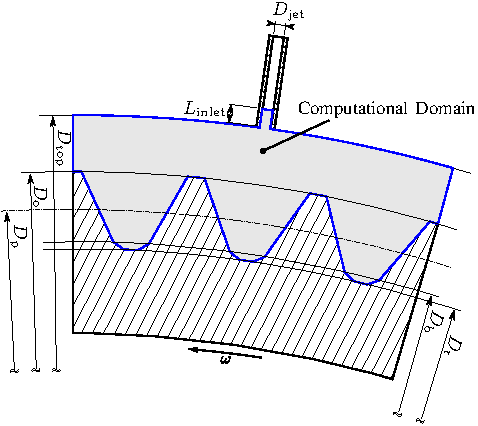
\includegraphics[width=0.7\textwidth]{bilder/keller_2016.pdf}
	\caption{Querschnitt durch das berechnete Segment des Zahnrads, \cite{keller2016}}
	\label{GRAPHIC:DomainKeller}
\end{figure}

% Die Platzierung der Abbildungen in figure-Umgebung kann anhand Optionen gesteuert werden:
% h - Die Abbildung wird wenn möglich an der Stelle der Definition eingefügt
% t - Die Abbildung wird oben auf der Seite platziert
% b - Die Abbildung wird unten auf der Seite platziert
% p - Eine eigene Seite mit Abbildungen wird angelegt
% Die Angabe von \begin{figure}[htbp] gibt die Priorität an. Zuerst wird versucht die Grafik an Ort und Stelle zu erzeugen. Gelingt dies nicht wird sie oben auf der Seite eingefügt, usw.

% Per \subcaptionbox können Abbildungen nebeneinander platziert und mit a), b) beschriftet werden
%\begin{figure}[ht]
%	\centering
%	\subcaptionbox{}{\includegraphics[width=0.48\columnwidth]{bilder/Bild_1_von_2}}\hfill
%	\subcaptionbox{}{\includegraphics[width=0.48\columnwidth]{bilder/Bild_2_von_2}}
%	\caption{GRAPHICS PLACED SIDE BY SIDE AND AMONG EACH OTHER WITH SUBORDINATE CAPTIONS}
%	\label{figure:_several_graphics}
%\end{figure}

Abbildungen helfen dem Autor, seine Erkenntnisse zu erläutern oder zu belegen. Diese Verbindung zwischen Abbildung und Aussage muss deutlich werden, sonst ist die Abbildung zu streichen. Alle Grafiken, Abbildungen und Tabellen müssen im Text referenziert und besprochen werden. Die Referenz ist durch eine fortlaufende Nummerierung der Objekte eindeutig vorzunehmen. Dabei werden Objekte gleichen Typs wie z.B. Abbildungen, Gleichungen und Tabellen jeweils gesondert nummeriert. Auf ein einheitliches Erscheinungsbild und Lesbarkeit achten (Textgröße, Auflösung, Größe angepasst an DIN A4, Vektorgrafiken wenn möglich). Abbildungen, die nicht selbst erstellt wurden, müssen ebenfalls zitiert werden. Wenn sie verändert wurden: \glqq Abbildung nach \cite{schoof2014}\grqq. Im Gegensatz zu Abbildungen besitzen Tabellen keine Unter- sondern Überschriften (siehe Tabelle \ref{tab:experiment-parameters}). Die Unterschriften sind möglichst aussagekräftig und eindeutig zu gestalten. Weitere Tabellenbeispiele werden von Markus Püschel\footnote{\url{https://www.inf.ethz.ch/personal/markusp/teaching/guides/guide-tables.pdf}} aufgezeigt. 

% Simple Beispiel-Tabelle
%\begin{table}[h]
%	\centering
%	\captionabove{Eine sinnlose Tabelle}
%	\begin{tabular}{|c|c|c|}
%		\hline
%		Spalte 1 & Spalte 2 & Spalte 3 \\
%		\hline
%		1 & 2 & 3 \\
%		\hline
%		1 & 2 & 3 \\
%		\hline
%		1 & 2 & 3 \\
%		\hline
%	\end{tabular}
%	\label{tab:test}
%\end{table}


\begin{table}[htbp]
	\centering
	\renewcommand{\arraystretch}{1.3} % Größerer Zeilenabstand
	\captionabove{Für die Modellierung verwendete Randbedingungen}
	\begin{tabular}{@{}lll@{}}
		\toprule
		Parameter           &   Variable   &           Value            \\ \midrule
		Hot gas temperature & $T_\text{h}$ &     \SI{490}{\kelvin}      \\
		Coolant temperature & $T_\text{c}$ &     \SI{270}{\kelvin}      \\
		Inlet Re            &     $Re$     &      $4.66\times10^5$      \\
		Inlet Velocity      & $u_\text{h}$ & \SI{33}{\meter\per\second} \\
		Tu Intensity        &     $Tu$     &     \SI{10}{\percent}      \\
		Operating Points    &     $DP$     &             1              \\ \bottomrule
	\end{tabular}
	\label{tab:experiment-parameters}
\end{table}


\newpage

\section{Diagramme}
\label{SECTION:Diagramme}

Alle gezeigten Diagramme sollten ein einheitliches Erscheinungsbild aufweisen. Achsen sind im Allgemeinen mit der physikalischen Größe und ihrer Einheit sowie Werte der physikalischen Größe zu beschriften. Schriftzeichen in Diagrammen sind ungefähr so groß wie im Text. Skalierung der Achsen sinnvoll wählen, um leeren Raum im Diagramm zu vermeiden. Es ist unter Umständen sinnvoll, die Skalierung einer Achse über mehrere Diagramme hinweg gleich zu wählen, wenn die Daten in den Diagrammen vergleichbar sein sollen (siehe Abbildung~\ref{fig:several_graphics}). Eventuell ist auch eine logarithmische Auftragung sinnvoll. Diagramme besitzen eine Legende. Sinnvolle min./max. Werte festlegen (nicht 0,2845 bis 9,385, sondern besser 0 bis 10). Ein Raster (\glqq grid\grqq) kann hilfreich sein. Diagramme farblich so gestalten, dass sie auch in schwarzweiß lesbar sind. In Abbildung \ref{fig:several_graphics} sind neben der farblichen Gestaltung zusätzlich unterschiedliche Marker und Linienarten eingesetzt. In der Regel ist der Hintergrund weiß, Sonderformatierungen (Hintergründe, Schriftarten) sind nur einzusetzen, wenn Vorteile daraus entstehen. Bei der Farbgebung auf die Erscheinungsform achten, zum Beispiel unterscheidet sich die Darstellung auf dem Beamer von der einer schriftlichen Ausarbeitung. Diagramme besitzen keinen alles umschließenden Rahmen. Abbildung möglichst einfach und leicht verständlich gestalten, in der Regel nicht mehr als drei Linien im Diagramm.

\begin{figure}[htpb]
	\centering
	\subcaptionbox{$x = \SI{0,7}{\mm}$} {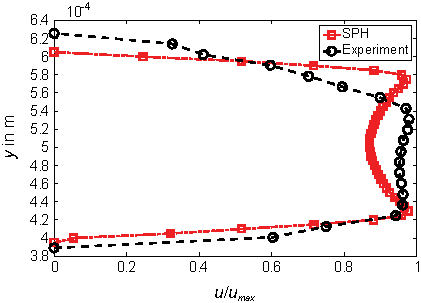
\includegraphics[width=0.48\columnwidth]{bilder/wieth_2016_2_6}}\hfill
	\subcaptionbox{$x = \SI{1,0}{\mm}$}{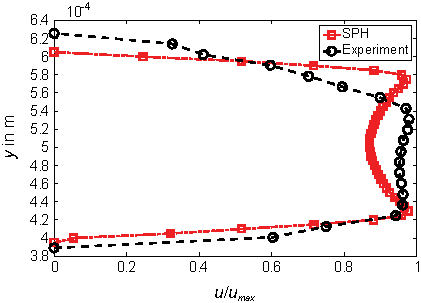
\includegraphics[width=0.48\columnwidth]{bilder/wieth_2016_2_6}}
	\subcaptionbox{$x = \SI{1,1}{\mm}$} {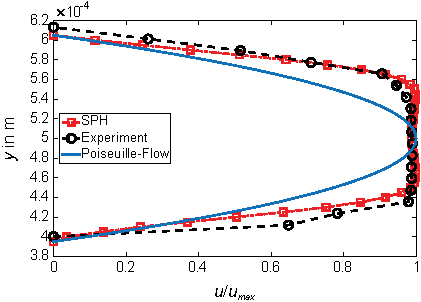
\includegraphics[width=0.48\columnwidth]{bilder/wieth_2016_3_6}}\hfill
	\subcaptionbox{$x = \SI{2.0}{\mm}$}{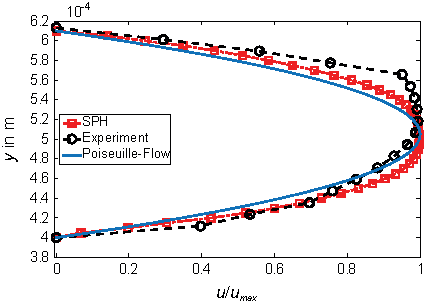
\includegraphics[width=0.48\columnwidth]{bilder/wieth_2016_4_6}}
	\subcaptionbox{$x = \SI{2,5}{\mm}$} {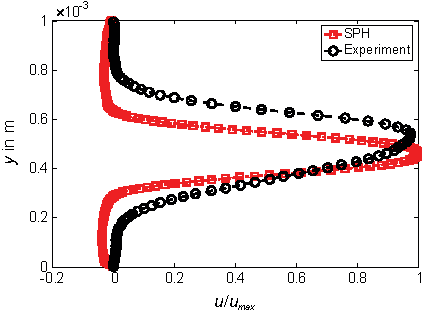
\includegraphics[width=0.48\columnwidth,height=5.5cm]{bilder/wieth_2016_5_6}}\hfill
	\subcaptionbox{$x = \SI{3,0}{\mm}$}{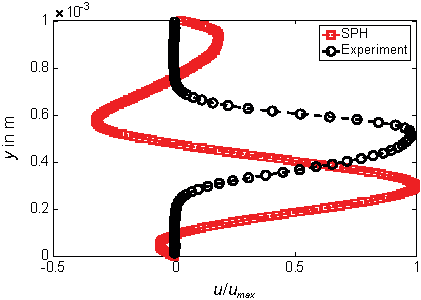
\includegraphics[width=0.48\columnwidth, height=5.5cm]{bilder/wieth_2016_6_6}}
	\caption{Vergleich zwischen experimentellen (kreisförmig) und berechneten (quadratisch) Werten, modifiziert nach \cite{wieth2016}. Da die Diagramme aus einer englischen Veröffentlichung stammen, sind die Dezimaltrennzeichen fälschlicherweise Punkte}
	\label{fig:several_graphics}
\end{figure}

\clearpage

\section{Gleichungen}
\label{SECTION:Gleichungen}

Alle Formelzeichen, die in einer Gleichung auftreten und nicht schon im vorangehenden Text definiert wurden, sind zu benennen und zu erläutern. In der Literatur etablierte Formelzeichen zur Beschreibung von physikalischen Größen wählen. Ein Formelzeichen beschreibt genau eine physikalische Größe. Jede physikalische Größe wird mit genau einem Formelzeichen beschrieben. Der Übersichtlichkeit halber mit Indizes und eingängigen Namen arbeiten. Gleichungen werden zentriert, nummeriert und sind Teil eines Satzes (besitzen also Satzzeichen). Zum Beispiel beschreibt der Impulssatz der Strömungsmechanik,

\begin{equation}
\label{EQUATION:Impuls}
\sum\vec{F}=\frac{d\vec{I}}{dt}=\underbrace{\frac{\partial}{\partial t}\iiint\varrho\:\vec{w}\:dV}_{\text{instationär}} + \underbrace{\iint\varrho\:\vec{w}\:\left(\vec{w}\cdot\vec{n}\right)\:dA}_{\text{stationär}},
\end{equation}

die zeitliche Änderung des Impulses $\frac{d\vec{I}}{dt}$ innerhalb eines Kontrollvolumens $V$, mit  der Dichte $\varrho$, dem Geschwindigkeitsvektor $\vec{w}$, der Oberfläche $A$ und dem äußeren Oberflächennormalen-Einheitsvektor $\vec{n}$. Die Änderung des Impulses entspricht der Summe der äußeren Kräfte $\sum\vec{F}$.

Formelzeichen werden immer zusammen mit einer Bezeichnung erwähnt. Die Angabe des Werts einer physikalischen Größe erfolgt immer mit der entsprechenden Einheit:

\begin{quote}
	$\Delta T$ = \SI{452,69}{\kelvin}.
\end{quote}

Zwischen Größe und Einheit, wie \SI{2,0}{\mm}, wird ein halbes Leerzeichen gesetzt (umbruchgeschütztes Leerzeichen verwenden bzw. \LaTeX-Paket siunitx). Einheiten und Operatoren, wie \glqq log\grqq, werden nicht kursiv gesetzt. Innerhalb der Arbeit auf eine einheitliche Darstellung für Vektoren, Tensoren etc. achten und SI-Einheiten verwenden.

%Formeln über mehrere Zeilen können zum Beispiel so realisiert werden:
%\begin{eqnarray}
%\sigma_e & = & n_0 \pi r^2 \xi_e \nonumber \\
%\sigma_s & = & n_0 \pi r^2 \xi_s \\
%\sigma_a & = & \sigma_e - \sigma_a
%\end{eqnarray}
% & richtet die einzelnen Zeilen zueinander aus.

%\section {Some text}
%TeX does not mean only programing and using commands. Examining the source-code of the text below, you will realise that typing a bigger paragraph of text is relatively simple and does not require more effort for formatting than with other programs. In the text-section below, among other things, some examples for font formatting and referencing are given.
%
%Fig.~\ref{figure:_zeilenumbruch} shows selected results of the LDV measurements of the gaseous 
%phase. In the upper diagram the phase averaged temporal 
%variation of the vertical component (axial velocity) 
%$u_{G,Y}(\phi)=\overline{u}_{G,Y}+u'_{G,Y}(\phi)$ is presented for a pulsating gaseous flow at a constant excitation 
%frequency of $f_S=\SI{250}{Hz}$, different mean velocities $\overline{u}_G$ and a constant 
%bypass setting of the siren. Apparently, the instantaneous 
%velocity $u_{G,Y}(\phi)$ is increasing with the mean velocity $\overline{u}_G$. However, the 
%relation is not proportional. There is a loss of velocity due to the positioning of the 
%LDV measuring volume in the wake of the prefilming surface and the divergence of the open jet. 
%Furthermore, the phase shift 
%is moving towards an earlier time at higher mean velocities. This can be explained by 
%the longer wavelength $\lambda \approx \overline{u}_G/f_S$ of the convected pulsation.
%It has to be noted that the signals are not perfectly sinusoidal 
%as anticipated. The fundamental mode is superimposed by a 
%first and second harmonic oscillations and additional noise. However, 
%those perturbing components represent only a fraction of the 
%designated signal.

%%%%%%%%%%%%%%%%%%%%%%%%%%%%%%%%%%%%%%%%%%%%%%%%%%%%%%%%%%%%%%%%%%%%%%%
% Literaturverzeichnis und Anhang
%%%%%%%%%%%%%%%%%%%%%%%%%%%%%%%%%%%%%%%%%%%%%%%%%%%%%%%%%%%%%%%%%%%%%%%
% Literaturverzeichnis auf einer ungeraden (rechten) Seite starten !
\cleardoublepage
%%%%%%%%%%%%%%%%%%%%%%%%%%%%%%%%%%%%%%%%%%%%%%%%%%%%%%%%%%%%%%%%%%%%%%
%  Literaturverzeichnis
%%%%%%%%%%%%%%%%%%%%%%%%%%%%%%%%%%%%%%%%%%%%%%%%%%%%%%%%%%%%%%%%%%%%%%
\refstepcounter{dummy}
\addcontentsline{toc}{chapter}{\refname}
%% Verschiedene Zitationsstile
% ITS
\bibliographystyle{literatur/itsBibStyle}
% Sonstige
%\bibliographystyle{plaindin}
%\bibliographystyle{unsrtdin}
%\bibliographystyle{abbrvdin}
%\bibliographystyle{alphadin}

%%%%%%%%%%%%%%%%%%%%%%%%%%%%%%%%%%%%%%%%%%%%%%%%%%%%%%%%%%%%%%%%%%%%%%
\bibliography{literatur/beispiel}

% Auf ungerader Seite starten
\cleardoublepage
%%%%%%%%%%%%%%%%%%%%%%%%%%%%%%%%%%%%%%%%%%%%%%%%%%%%%%%%%%%%%%%%
% Anhang
%%%%%%%%%%%%%%%%%%%%%%%%%%%%%%%%%%%%%%%%%%%%%%%%%%%%%%%%%%%%%%%%
\appendix
\chapter*{\appendixname}
\stepcounter{chapter}
\addcontentsline{toc}{chapter}{\appendixname}		% Name des Anhangs in Inhaltverzeichnis auf Kapitelebene schreiben
\ihead{\appendixname}								% Kopfzeile setzen

%%%%%%%%%%%%%%%%%%%%%%%%%%%%%%%%%%%%%%%%%%%%%%%%%%%%%%%%%%%%%%%%
\section{Anhang 1}
\begin{table}[htbp]
	\centering
	\renewcommand{\arraystretch}{1.3} % Größerer Zeilenabstand
	\captionabove{Simulationsergebnisse, die den Lesefluss stören.}
	\begin{tabular}{@{}rrrrcrrr@{}}
		\toprule
		&\multicolumn{3}{c}{$w = 8$} & \phantom{abc}& \multicolumn{3}{c}{$w = 16$}  \\
		\cmidrule{2-4} \cmidrule{6-8}
		& $t=0$ & $t=1$ & $t=2$ && $t=0$ & $t=1$ & $t=2$  \\
		\midrule
		$dir=1$ \\
		$c$ & 0,0790 & 0,1692 & 0,2945 && 0,3670 & 0,7187 & 3,1815 \\
		$c$ &  -0,8651& 50,0476& 5,9384&& -9,0714& 297,0923& 46,2143\\
		$c$ & 124,2756& -50,9612& -14,2721&& 128,2265& -630,5455& -381,0930\\
		$dir=0$\\
		$c$ & 0,0357& 1,2473& 0,2119&& 0,3593& -0,2755& 2,1764\\
		$c$ & -17,9048& -37,1111& 8,8591&& -30,7381& -9,5952& -3,0000\\
		$c$ & 105,5518& 232,1160& -94,7351&& 100,2497& 141,2778& -259,7326\\
		\bottomrule
	\end{tabular}
	\label{tab:example-table}
\end{table}
\section{Anhang 2}
\lipsum

\end{document}
